\section{Evaluation} \label{Eval}
The evaluation chapter takes the theoretical background from the previous chapters and puts them to practical use.
Here the parameters from the Long Short-Term Memory models get tested and analyzed for the best values.
From these parameters a model is build and tested against an Auto-Regressive Integrated Moving Average model.

\subsection{Test Data}
As described in Section \ref{chooseDataset} the chosen dataset is the data from the GÉANT network.
Figure \ref{fig:geanttopologymapdecember2018image} shows the topology of the network\footnote{\url{https://www.geant.org/Networks/Pan-European_network/Pages/GEANT_topology_map.aspx} Accessed: 2019-11-21}.
In the dataset all communication pairs are included.
So communication between node 1 and 2, node 1 and 3, node 1 and 4 and so forth.
As test data for the evaluation five of these communication pairs were used.
The pairs are source 1 to 5 all to destination 11.
I cannot show the exact nodes in Figure \ref{fig:geanttopologymapdecember2018image} as the data I have was anonymized by the authors.
\begin{figure}
	\centering
	\includegraphics[trim={0in 6.7in 0in 5in}, width=1\linewidth, clip]{Pictures/GEANT_Topology_Map_December_2018}
	\caption{GÉANT network topology}
	\label{fig:geanttopologymapdecember2018image}
\end{figure}
Also described in a previous Section (\ref{datasetMod}) is how the data is interpreted.
I interpreted nodes 1 to 10 as services while the rest of the nodes I interpreted as the ingress nodes.
So, the five communication pairs are five different services accessing the node 11.
Each pair has a distinctly different pattern of communication.
The training data consists of 1199 values.
The library uses 999 of those values for training and the rest used for testing the models.
From the 999 values again, 20\% is used for validating the training steps.
This validation data is used to monitor training success.
If both the loss on the training and validation data is improving (getting smaller), that means the training is working.
If only the loss on the training data is improving, that means the model is overfitting on the training data\footnote{This means that the weights of the model are fitted too much for the values of the training set and the model loses the ability to predict other data.}.
To test the data after training, a third test set is used, that was not involved in the training of the model, to confirm the performance on the training and validation set.
For the hyperparameter optimization, the number of tests per configuration was 40 repetitions.
In the plots I removed the outliers, so the scale of the plots was not too big, but each box had not more than five outliers.
The majority hat less than two outliers.
All the experiments where the parameters combinations changed contain 40 repetitions.

\subsection{The LSTM Model}
The content of this section describes the construction of a model containing LSTM layers, how the data has to be modified, how to do hyperparameter optimization and what to look out for.
\subsubsection{Identifying the best Architecture and Parameters}\label{archParam}
For constructing an LSTM model, Keras provides an LSTM layer.
This layer implements an RNN LSTM layer with all the LSTM mechanisms all already implemented.
Keras provides many configuration possibilities for each layer.
The options for the LSTM layer include the number of hidden nodes, activation function, use of bias and so forth.
Because of the many possible configurations and the resulting complexity, I decided to keep the standard values of most parameters and tune the parameters that mostly influence the complexity of the layer, which in the case of the LSTM layer is the number of hidden units.

Also combining multiple LSTM layers creates a network with higher computation complexity.
First, the input and output are explained to understand better how to connect layers.
The input for the first LSTM layer in the architecture has the shape of (batch size, time-steps, features).
When retaking the example of the sequence [1,2,3,4,5] and using two values to predict the third value: our input-array when using the Keras would look like this:
\begin{displayquote}
	$[[1, 2]$\linebreak
	$ [2, 3]$\linebreak
	$ [3, 4]]$
\end{displayquote}
The pair 4,5 is left out because there exists no corresponding result.
Keras splits the array apart and feeds the LSTM with the sequences of 1,2 / 2,3 / 3,4 , when each batch has the size of one.
Of course, also fed into the model is the corresponding third number as a target for the training.
Usually, the output of the LSTM would be of the shape (batch size, units) (units meaning the hidden nodes), as can be seen in Figure \ref{fig:singlelstmkeras} a).
However, when constructing the network, one has to pay attention to setting the parameter \textit{return\_sequence} to true.
This results in a new output with an extra dimension containing all predictions, not just the final one so that the LSTMs can connect as in Figure \ref{fig:unrolled2layerlstm}.            
\begin{figure}
	\centering
	\includegraphics[width=0.7\linewidth]{Pictures/SingleLSTMKeras}
	\caption{Examples of how Keras sets up LSTMs and how the inputs and outputs are shaped.}
	\label{fig:singlelstmkeras}
\end{figure}

As described before, the output of an LSTM layer has the dimension (batch size, units).
This is not the one value we want from the prediction.
To get one definitive result in Keras the vector with the size of units has to be reduced to one output, which is done using a \textit{Dense} layer.
The \textit{Dense} layer is a basic neural network layer that connects all inputs to a defined number of outputs, for example, one value.            

As two examples for two implementations: the original paper that introduced LSTM did not yet have a forget gate \cite{lstmOrig}, the forget gate was introduced later in \cite{iet:/content/conferences/10.1049/cp_19991218}.

As described in Section \ref{training}, the optimizer and loss function are also an essential factor in the training of a neural network.
For the testing, I decided to stay with the \textit{Mean Squared Error} loss function, as it is a simple and effective way of judging the quality of the training.
Furthermore, I chose the ADAM optimizer, as it is also an often used and standard optimizer.

For the actual testing of the models, an extra library is used, called \textit{Talos}.
Apart from the hyper-parameter optimization, \textit{Talos} has the bonus that the library stores all training results from each parameter combination in a .csv file for easy analysis.

\subsubsection{Training the LSTM}
The input of a neural network during the training is always an input array and a corresponding array with targets that the model should predict.

\begin{figure}
	\centering
	\includegraphics[width=0.5\linewidth]{Pictures/LSTM_Training}
	\caption{How the arrays are created for the training of an LSTM.}
	\label{fig:lstmtraining}
\end{figure}

In the example in Figure \ref{fig:lstmtraining} the sequence 1 to 10 is transformed into an input array X and a goal array Y.
For this example the number of previous values used for a prediction is two.
That is why the array X has two columns.
Usually, the input array would need three dimensions for an RNN model in Keras.
The third dimension would be the feature dimension.
Since there exists only one feature, I omitted the dimension in this example.

\subsubsection{Hyperparameter-Tuning Results}
\begin{figure}
	\centering
	\includegraphics[width=1\linewidth]{Pictures/Results/experiment_1_1_1}
	\caption{The loss and validation loss when increasing the number of hidden nodes for pair (1,11).}
	\label{fig:experiment_1}
\end{figure}
The next section describes the results from tests with hyperparameter optimization using the data described before.

\paragraph{Hidden Nodes}
First, the effect of the number of hidden nodes was analyzed.
This parameter describes the number of hidden nodes per LSTM layer.
As can be seen in Figure \ref{fig:experiment_1} increasing the number of hidden nodes results in a higher probability that the network will produce low error predictions.
The same can also be seen with the validation loss.
However, when increasing the epochs (more training steps), the advantage for the higher number of nodes vanishes and all models perform the same (Figure \ref{fig:experiment_1}).
The shrinking advantage is an important fact because the training time can increase drastically when using a high number of hidden nodes, especially when combining multiple layers.
This pattern can also be seen with all the five different pairs Figure \ref{fig:experiment_1_1_3} to \ref{fig:experiment_1_1_5} in the Appendix.
Except for the validation loss in Figure \ref{fig:experiment_1_1_2}, here, the validation loss stays constant over the increasing number of hidden nodes and epochs.
I suspect that the results look like this, since the model is only predicting one value.
When using an output vector with more than one value and the resulting higher number of weights and more complex calculation hold only a small benefit when predicting only one value.
Due to the unique traffic pattern of the pair (2,11), the pair is not reacting as well to the changes as the other time-series.
I further analyze the pattern in section \ref{optimization}.

\paragraph{Previous Values}
Another important parameter is how many values to take into account when predicting a new value; utilizing one of the essential features of the LSTMs, the passing of prediction and cell-state to the next step as in Figure \ref{fig:unrolled2layerlstm}.
When looking at the test in Figure \ref{fig:experiment_2}, the advantage of using multiple previous values becomes apparent.
For the validation set an advantage can be seen until using 4 previous values, after that the loss function stalls.
Nevertheless, when increasing the epochs in Figure \ref{fig:experiment_2} it also becomes clear, that models with more than one step suffer from severe overfitting.
The loss from the training set, trained with 1000 epochs, shrinks drastically, while the loss for the validation set increases.
That shows that a model that uses multiple past steps is more sensitive to the training data.
This could be because there exist fewer commonalities between the training data and the validation data and how they relate to their previous values.
In short the rules that produce $x_3$ from $x_1$ and $x_2$ have only few correlations with the rules that produce $y_3$ from $y_1$ and $y_2$ with $y_3,y_2,y_1\in Validation Set$ and $x_3,x_2,x_1\in Training Set$.
So, these results show that when training the LSTM with multiple previous values, one must pay attention as it can lead to severe overfitting.
\begin{figure}
	\centering
	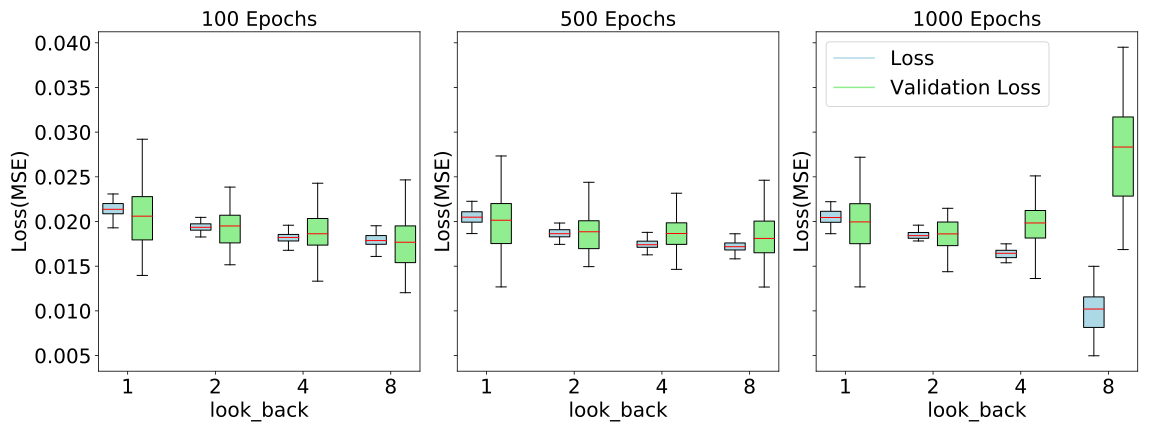
\includegraphics[width=1\linewidth]{Pictures/Results/experiment_2_1_1}
	\caption{The loss and validation loss when increasing the number of previous values to take into 
		account for a prediction for pair (1,11).}
	\label{fig:experiment_2}
\end{figure}

\paragraph{Number of Batches}
In Keras the parameter that controls the number of batches is called \textit{batch\_size}, this parameter indirectly controls the size of the batches by defining how many batches are created.
So, through increasing the number of batches (fewer values per batch) in Figure \ref{fig:experiment_4}, it is clear that with smaller batches you need a much higher number of epochs to get the same result.
This occurs because in each epoch only one randomly chosen batch is shown to the model for training, so to get an equal coverage of the data it takes more epochs.
The plots show that at some point smaller batches perform at least as good as the one big batch, but a lot more epochs are needed.
However, one big batch also takes a lot longer to compute than one small batch per epoch, so a trade-off has to be found between computation time per epoch and number of epochs.
\begin{figure}
	\centering
	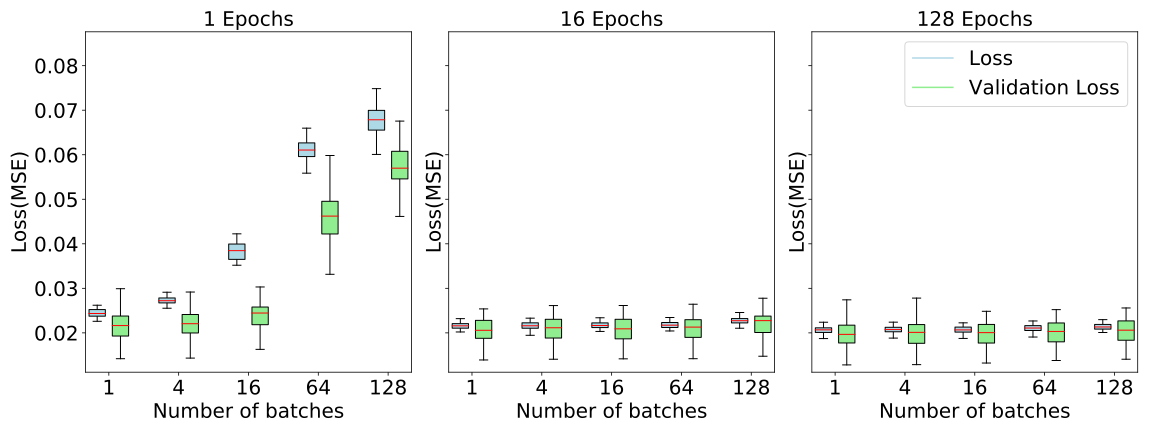
\includegraphics[width=1\linewidth]{Pictures/Results/experiment_4_1}
	\caption{The impact of epochs vs. number of batches for pair (1,11).}
	\label{fig:experiment_4}
\end{figure}

\paragraph{LSTM Layers}
The last parameter tested was how the number of LSTM layers influence the prediction error; the layers are stacked just like in Figure \ref{fig:unrolled2layerlstm}.
The plot in Figure \ref{fig:experiment_3} shows that more layers only slightly improve the predictions and and this is not the case for the other pairs (Figure \ref{fig:experiment_3_2} to Figure \ref{fig:experiment_3_5}).
This advantage also disappears further, when increasing the number of training epochs beyond 100.
These plots show that in this application, the number of layers is playing a small role and one can completely disregard it when using enough epochs.
This could be because the extra layers have the same number of hidden nodes in them like the previous ones and perform predictions based on predictions with the same complexity in each layer.
A possible improvement could be the increase in complexity in the extra layers.

\begin{figure}
	\centering
	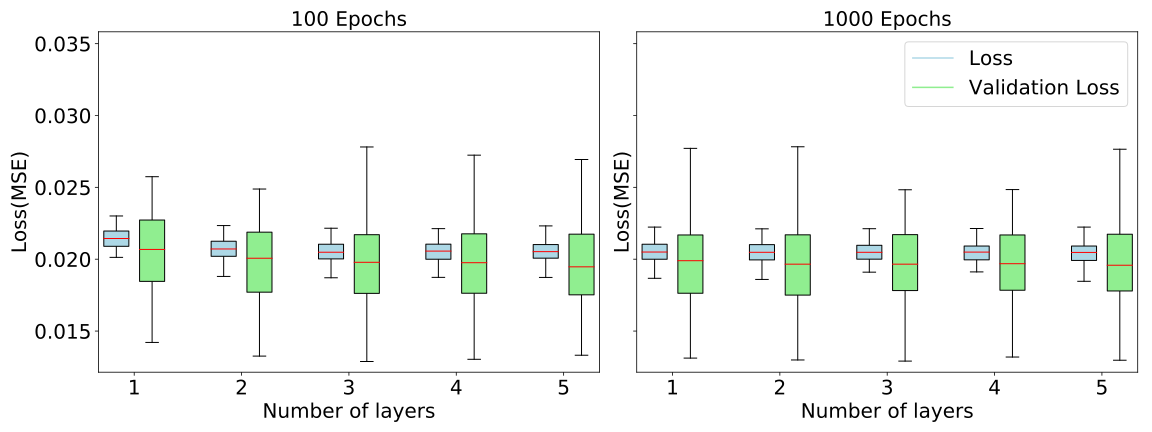
\includegraphics[width=1\linewidth]{Pictures/Results/experiment_3_1}
	\caption{Plot of how the number of LSTM layers influence the loss and validation loss for pair (1,11).}
	\label{fig:experiment_3}
\end{figure}

Now using all the test results, I can build a model that can predict the traffic.
Since the test results were so similar, even one hyperparameter setting could work for all communication pairs.
The plots in Figure \ref{fig:experiment_3} show that the model can use only one layer without it harming the predictions.
The exception for this is the first communication pair.
To get an equally good prediction for the first pair the number of epochs is chosen to be 1000.
Also, the high number of epochs has only a negative effect when the model uses more than two previous values (look\_back in the plot) , so the look\_back is going to be two for the model.
To speed up the training, since the model is training with 1000 epochs, I chose a batch size of 128.
Furthermore, only one hidden node is selected, as more nodes do not bring an advantage.

Using this model trained for 1000 epochs produces results that Figure \ref{fig:LSTMpredictions} shows.
The rest can be seen in the Appendix in Figure \ref{fig:LSTMprediction_0} to \ref{fig:LSTMprediction_4}.
The test set contains the 200 most current values, and the models have never seen these values.
The results vary from very good prediction (Figure \ref{fig:LSTMprediction_03}) to bad predictions (Figure \ref{fig:LSTMprediction_01}).
What the results seem to have in common is that they are good at predicting the rough shape of the traffic.
What all seem to struggle with is to get the exact values correct.      

\begin{figure}
	\centering
	\begin{subfigure}{1\linewidth}
		\centering
		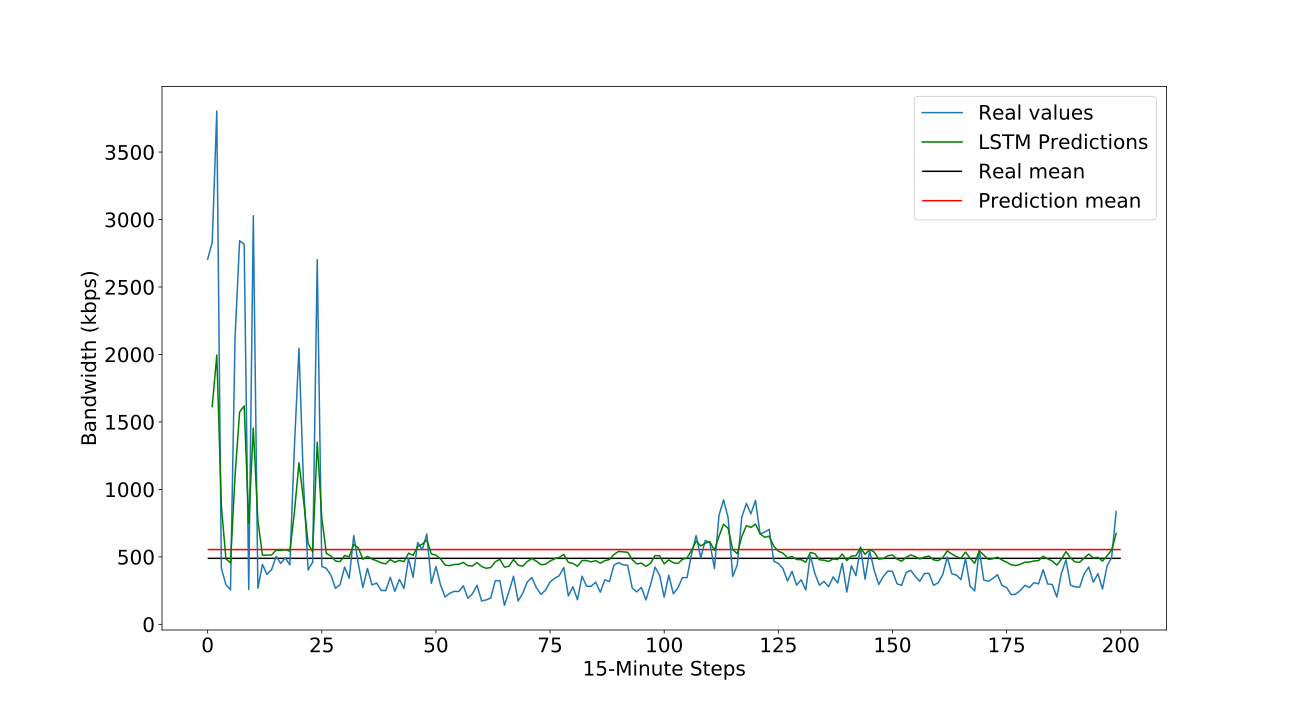
\includegraphics[width=1\linewidth]{Pictures/Practical_Examples/LSTMprediction_1}
		\caption{Pair (2, 11)}
		\label{fig:LSTMprediction_01}
	\end{subfigure}
	\begin{subfigure}{1\linewidth}
		\centering
		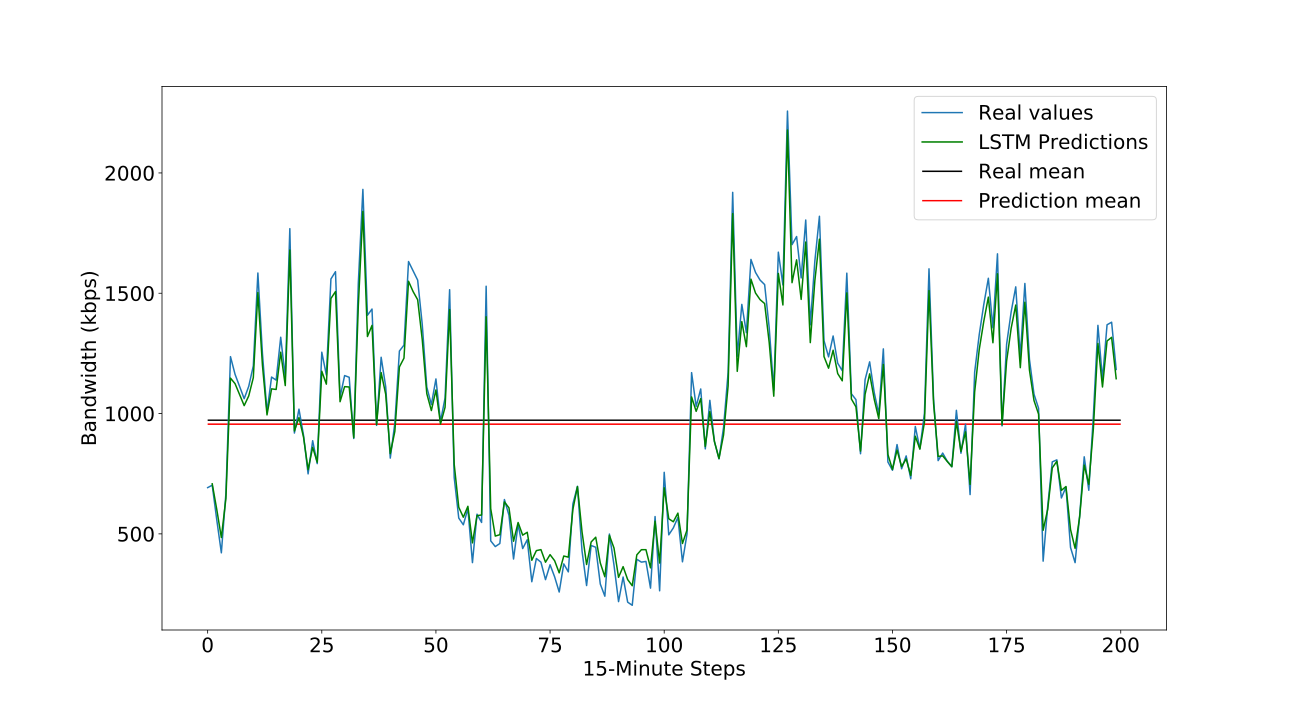
\includegraphics[width=1\linewidth]{Pictures/Practical_Examples/LSTMprediction_3}
		\caption{Pair (4, 11)}
		\label{fig:LSTMprediction_03}
	\end{subfigure}
	\caption{Prediction results of the traffic of pair (2,11) and (4,11).}
	\label{fig:LSTMpredictions}
\end{figure}

\subsection{The ARIMA Model}
Since I used the automatic ARIMA model builder, in this section, a short description is given on how the different chosen models look.

The values in the table below show the orders of the parts of the ARIMA model, chosen by the automatic ARIMA optimization.    

\begin{center}
	\begin{tabular}{|c|c|c|c|c|c|c|}
		\hline 
		source & p & d & q & P & D & Q \\ 
		\hline 
		1 & 1 & 1 & 2 & 0 & 0 & 0 \\ 
		\hline 
		2 & 3 & 0 & 3 & 2 & 0 & 1 \\ 
		\hline 
		3 & 2 & 0 & 2 & 0 & 0 & 0 \\ 
		\hline 
		4 & 1 & 1 & 2 & 0 & 0 & 1 \\ 
		\hline 
		5 & 3 & 0 & 3 & 2 & 0 & 2 \\ 
		\hline 
	\end{tabular}
\end{center}

When using these automatically optimized models two of the predictions of those models can be seen in Figure \ref{fig:ARIMAprediction1}, the rest can be seen in the Appendix in Figure \ref{fig:ARIMAprediction_0} to \ref{fig:ARIMAprediction_3}.
On first glance, these predictions look very similar to the LSTM predictions.
Of course, there exist some obvious errors that the LSTMs are not producing like the overcompensation in Figure \ref{fig:ARIMAprediction_4} at the 175th step.
Nevertheless, the models predict other parts of the traffic equally well.

\subsection{Comparing LSTM and ARIMA}    
Comparing all the errors from the ARIMA and the LSTM, the similarity in performance is undeniable.
Figure \ref{fig:BoxERRORprediction} shows the average error in the predictions of the test set.
Overall the LSTM is not much better than the ARIMA model.
What could be said, is that the LSTM is more consistent as it produces fewer outliers than the ARIMA.

\begin{figure}
	\begin{subfigure}{1\linewidth}
		\centering
		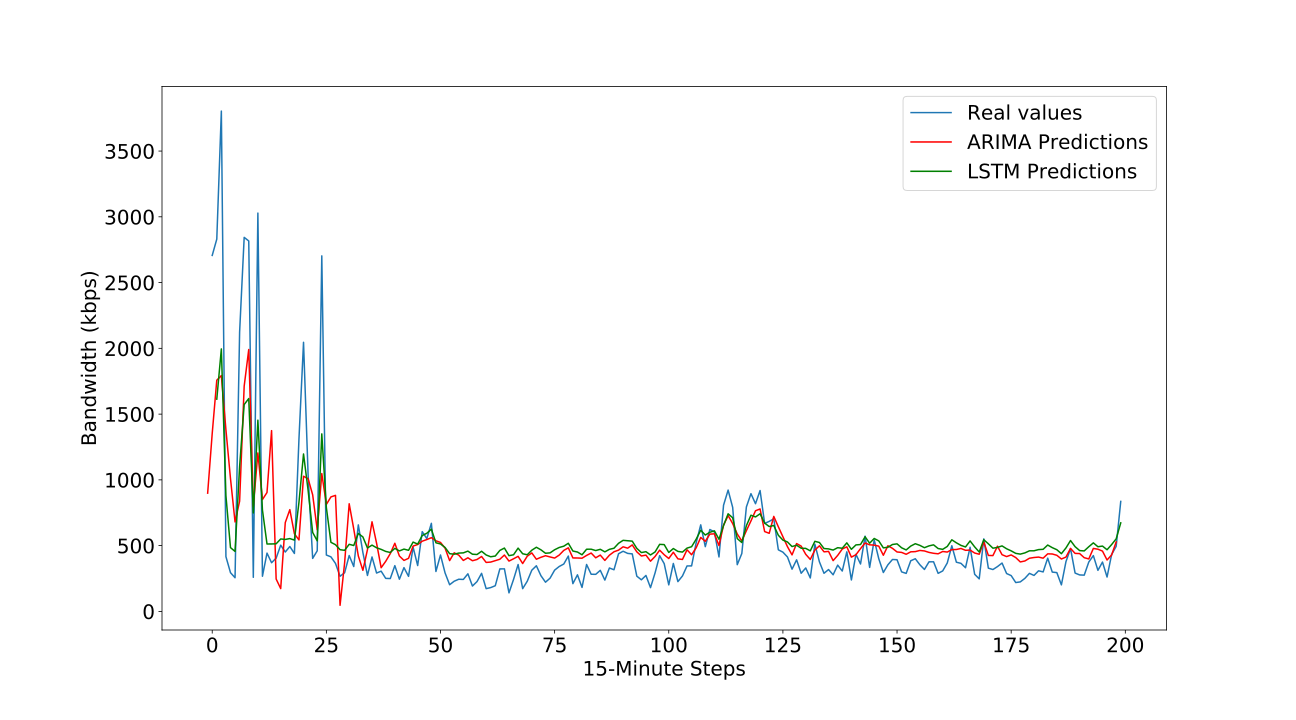
\includegraphics[width=1\linewidth]{Pictures/Practical_Examples/AvLprediction_1}
		\caption{Pair (2, 11)}
		\label{fig:ARIMAprediction_1}
	\end{subfigure}
	\begin{subfigure}{1\linewidth}
		\centering
		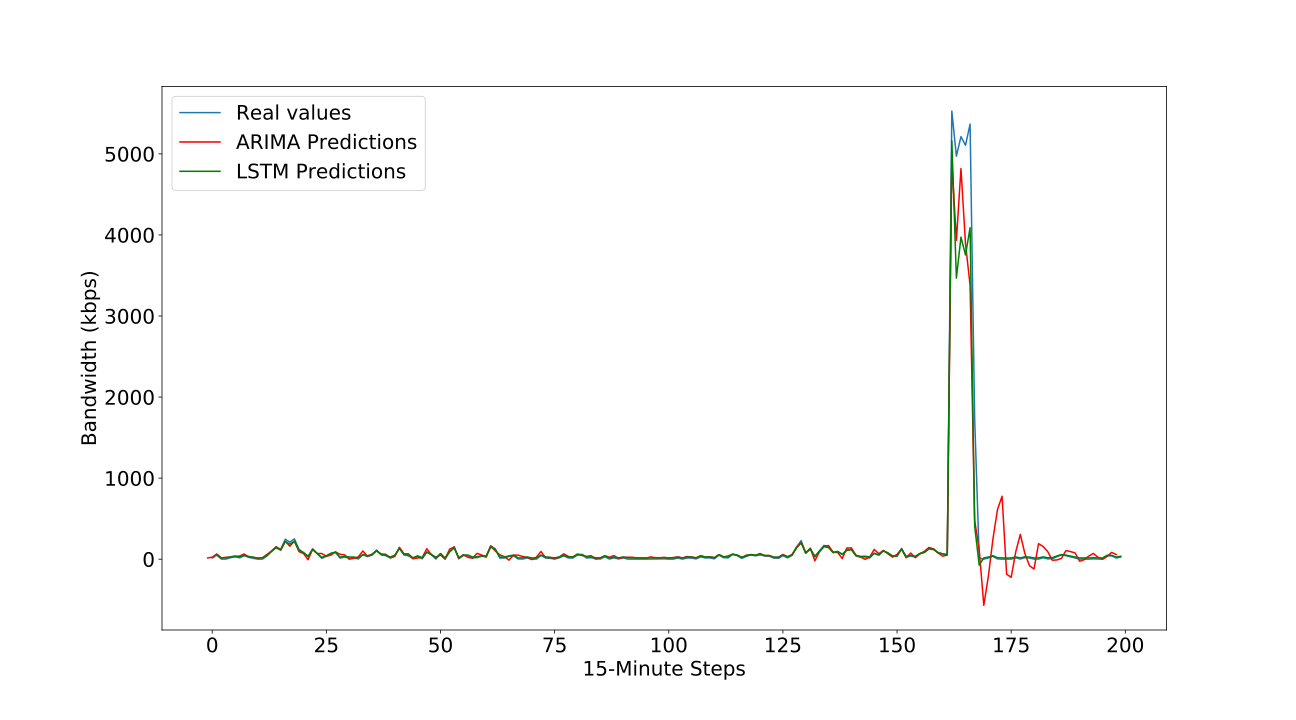
\includegraphics[width=1\linewidth]{Pictures/Practical_Examples/AvLprediction_4}
		\caption{Pair (5, 11)}
		\label{fig:ARIMAprediction_4}
	\end{subfigure}
	\caption{Predictions of the ARIMA model vs the LSTM model.}
	\label{fig:ARIMAprediction1}
\end{figure}

\begin{figure}
	\centering
	\begin{subfigure}{0.42\linewidth}
		\centering
		\includegraphics[width=1\linewidth]{Pictures/Practical_Examples/BoxERRORprediction_0}
		\caption{Pair (1, 11)}
		\label{fig:BoxERRORprediction_0}
	\end{subfigure}
	\begin{subfigure}{0.42\linewidth}
		\centering
		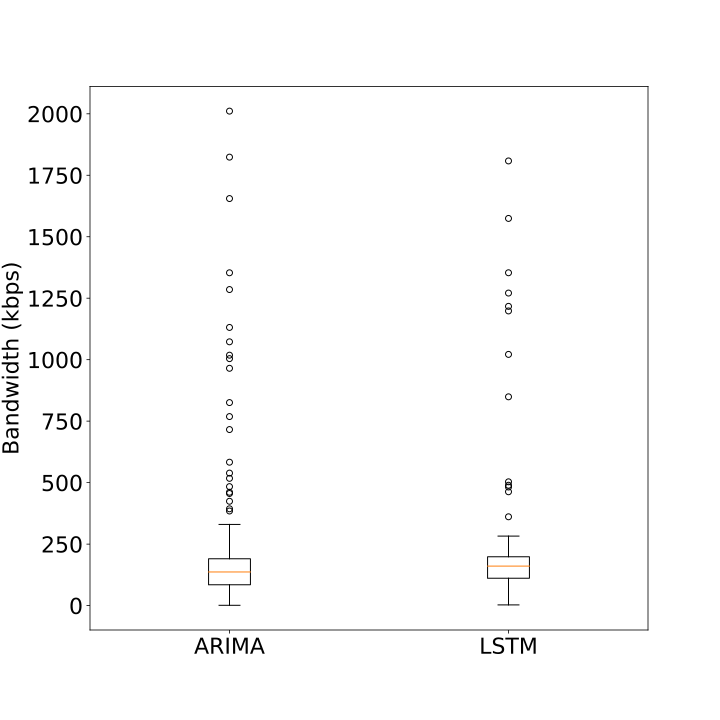
\includegraphics[width=1\linewidth]{Pictures/Practical_Examples/BoxERRORprediction_1}
		\caption{Pair (2, 11)}
		\label{fig:BoxERRORprediction_1}
	\end{subfigure}
	\begin{subfigure}{0.42\linewidth}
		\centering
		\includegraphics[width=1\linewidth]{Pictures/Practical_Examples/BoxERRORprediction_2}
		\caption{Pair (3, 11)}
		\label{fig:BoxERRORprediction_2}
	\end{subfigure}
	\begin{subfigure}{0.42\linewidth}
		\centering
		\includegraphics[width=1\linewidth]{Pictures/Practical_Examples/BoxERRORprediction_3}
		\caption{Pair (4, 11)}
		\label{fig:BoxERRORprediction_3}
	\end{subfigure}
	\begin{subfigure}{0.42\linewidth}
		\centering
		\includegraphics[width=1\linewidth]{Pictures/Practical_Examples/BoxERRORprediction_4}
		\caption{Pair (5, 11)}
		\label{fig:BoxERRORprediction_4}
	\end{subfigure}
	\caption{Comparison of the error in the prediction. ARIMA vs LSTM.}
	\label{fig:BoxERRORprediction}
\end{figure}

Also crucial for practical usage of the prediction models is how long they take to train and to predict a value.
This dictates how often the system can make a prediction and how fast an algorithm could react to future changes in the traffic.
Figure \ref{fig:BoxTraining} shows the times for training an LSTM model and fitting an ARIMA model.
The fitting of the ARIMA model is a lot faster than the training of the LSTM model.
I trained the LSTM model with 1000 epochs, so using only 100 epochs would get the LSTM training time closer to the ARIMA time, but that could only be done if it would not impair the prediction quality.

The second plot, Figure \ref{fig:BoxPrediction}, shows the differences between how long it takes a model to predict one value.
Included in the ARIMA time is the fitting of the model with the next value, as it is not usable if the model is not updated.
Here the LSTM has a clear advantage to the ARIMA model.
This is the case because for the LSTM the prediction is just calculating a few formulas with the previously found weights.
For the ARIMA, on the other hand, it is not just the calculation of the formulas but the refitting of the model with the new data.

These two plots show that one has to make a careful choice.
If the LSTM model needs to be retrained often, because the pattern of the data changes a lot, than the ARIMA has the clear advantage.
Especially if the LSTM model would get more complicated, the time for training would increase.
However, if the model does not have to be updated often, the LSTM performs much better than the ARIMA.

\begin{figure}
	\centering
	\begin{subfigure}{0.4\linewidth}
		\centering
		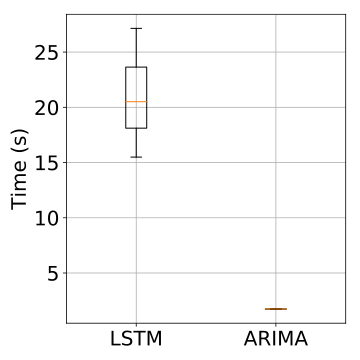
\includegraphics[width=1\linewidth]{Pictures/TimeComp/TrainingTime}
		\caption{The time needed for training/fitting the model}
		\label{fig:BoxTraining}
	\end{subfigure}
	\begin{subfigure}{0.4\linewidth}
		\centering
		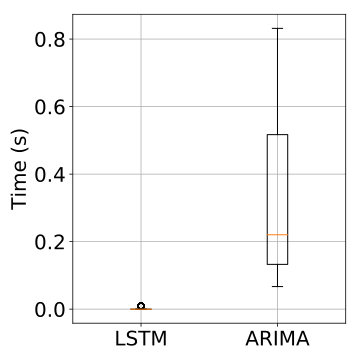
\includegraphics[width=1\linewidth]{Pictures/TimeComp/PredictionTime}
		\caption{The time needed for making a prediction of one value}
		\label{fig:BoxPrediction}
	\end{subfigure}
	\caption{Comparison of the relevant times measured for a LSTM and an ARIMA model}
	\label{fig:Times}
\end{figure}

With just these results, I cannot recommend using the LSTM over the ARIMA.
The performance on the prediction side is very similar, only decided by the lower number of outliers produced by the LSTM.
When looking at the time comparison, the LSTM is slower to train but faster at predicting values.
The only factor that distinguishes the two approaches is complexity.
One can automatically compute the ARIMA model after finding a suitable parameter m, number of periods in a season.
On the other hand, the LSTM model architecture allows for a vast number of different configurations and different parameter settings.
Finding the best parameters can also be done automatically via a hyperparameter optimization, but depending on the number of parameters and the computation resources available, the optimization can take up to a few days to complete.

\subsection{Optimizing LSTM Prediction}\label{optimization}
To analyze the predictions, I looked closer at the pair with the worst predictions, pair (2,11).
When looking at the prediction in Figure \ref{fig:LSTMprediction_01}, the predictions never go below a specific value.
Furthermore, the model predicts the majority of the values too high.
\begin{figure}
	\centering
	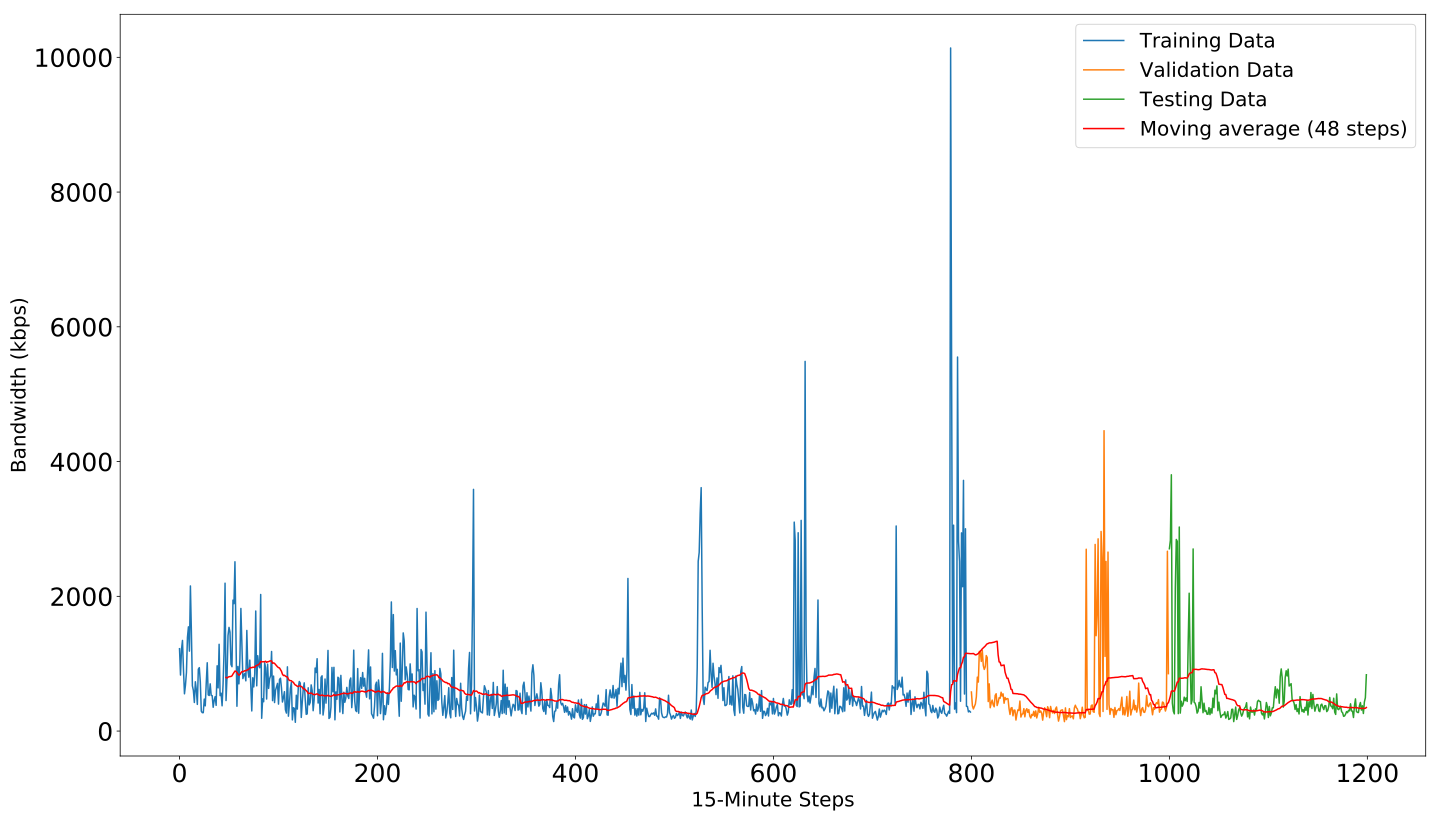
\includegraphics[width=0.95\linewidth]{Pictures/Traffic_Analysis/Traffic_rolling_average_2}
	\caption{The traffic from pair (2,11) used for training, validating and testing the model.}
	\label{fig:trafficrollingaverage2}
\end{figure}
Figure \ref{fig:trafficrollingaverage2} shows the traffic of the pair (2,11) and how it was split up into training, validation and testing data.
Also included in the Figure is the moving average over 48 steps, that is equivalent to 12 hours, so it is a 12-hour moving average.
In the first part of the data from step 0 to 400 the moving average shows a decline with two small spikes but no discernible pattern.
Looking further to the right after step 400, a pattern emerges.
There are bumps in the moving average of the length of roughly 100 steps.
The bumps continue until step 800 with a broader bump in the average.
After that broader bump, it continues with the spikes of width 100.
When seeing this pattern, maybe the prediction could be improved when omitting the first 400 steps that show no sign of the pattern.
Additionally, to omitting the 400 steps, the test includes multiple data ranges in 100 step steps, training with 100 steps, 200 steps and continuing this to 600 steps.
However, testing with the 600 steps that omit the 400 first steps has absolutely no influence on the prediction.
The model performs the same as with the 1000 steps.
What improved the model was training it with just 200 steps.
As can be seen in Figure \ref{fig:opti}, the predictions get closer to the actual real values.
This proves that the amount of training data fundamentally changes the ability of a model to make accurate predictions.
Also, this makes the models more challenging to use in a practical scenario as every model needs a different amount of data and a way of identifying how much data it needs.
What is also very important is that training the model with only 200 values made the training a lot more inconsistent.
The result in Figure \ref{fig:opti} is one of the better results, but the training could also result in a worse performance than training with the 1000 values.
\begin{figure}
	\centering
	\includegraphics[width=1\linewidth]{Pictures/optimization/LSTMoptimization_1_take2}
	\caption{Prediction when LSTM is trained with 200 values.}
	\label{fig:opti}
\end{figure}

\subsection{One-Step Prediction vs Multi-Step Prediction}
In this section two approaches are closer described that the ARIMA model can not replicate.
The first approach is the prediction of values more than one step in the future from the current value.
As mentioned earlier the ARIMA model can predict multiple values into the future at once, but anything beyond one value ahead has no usable accuracy.
Again using the example of the sequence [1,2,3,4,5], an example would be to predict the 4 based only on the sequence 1,2.
The training of the LSTM works the same as with the one-step prediction.
The input sequence stays the same, what changes are the target values.
These values are shifted by the number of values one wants to predict in the future.
\begin{figure}
	\centering
	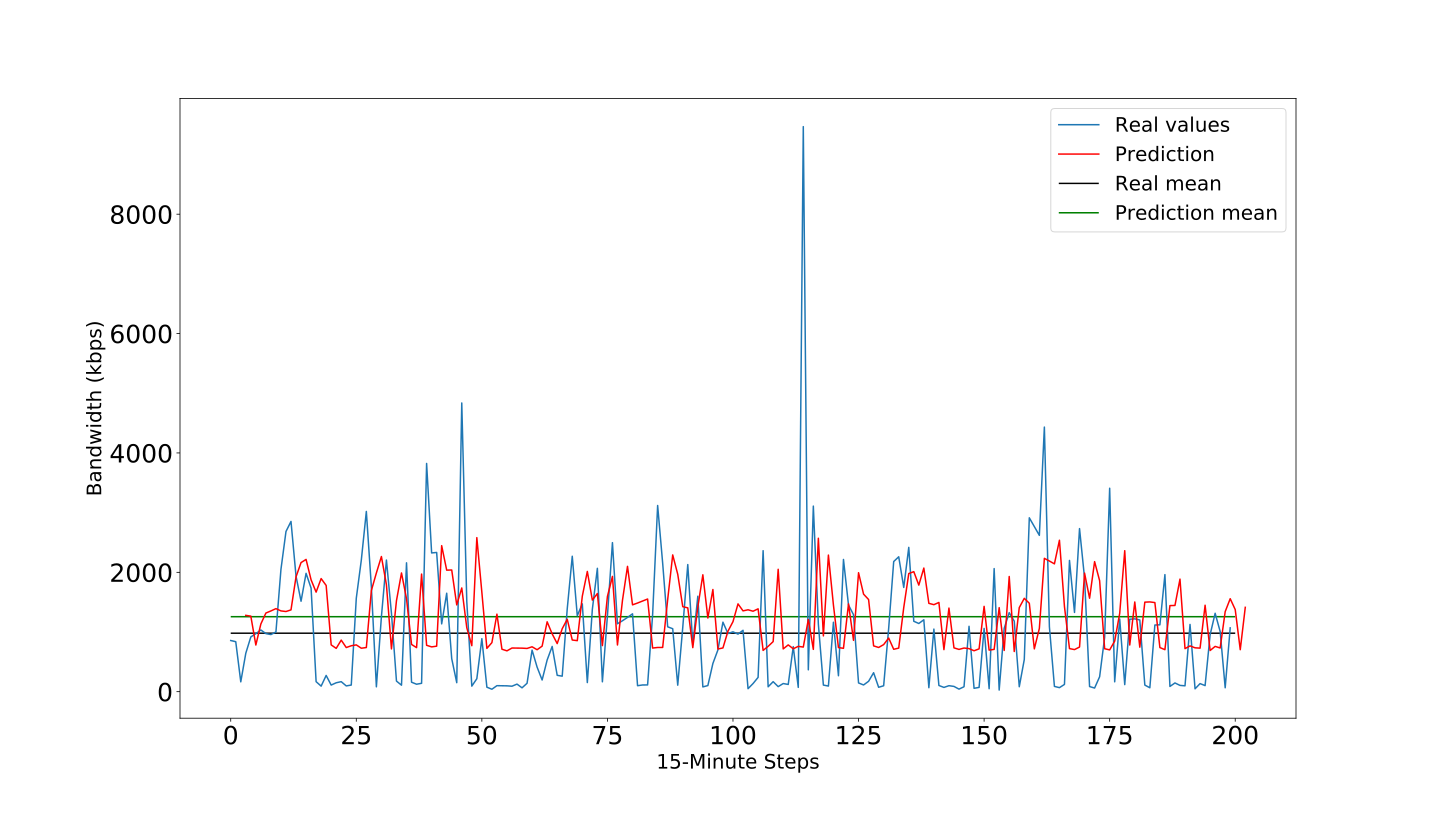
\includegraphics[width=1\linewidth]{Pictures/BigStep/LSTM_Big_Step_40}
	\caption{LSTM prediction, when trained with 4 steps into the future.}
	\label{fig:lstmbigstep0}
\end{figure}
But what happens when the LSTM is trained this way is displayed in Figure \ref{fig:lstmbigstep0}.
In this example the LSTM was trained to predict 4 values into the future with two previous values as input.
So, using two values to predict the next value in 4 steps.
But the LSTM not actually predicts the value in 4 steps but a shifted and squashed version of the next step.
So when inputting the value n-1 and n, instead of predicting n+4 the model predicted n+1 in a scaled down version.
This trend continues when predicting further into the future.
The squashing of the prediction continues until it approaches the mean of the one-step prediction.
In Figure \ref{fig:bigStep1} this trend can be observed as the prediction of 16 steps into the future represents the mean of the predictions one step into the future.

The same phenomenon can be observed when trying to teach the LSTM to predict a range of future values instead of just one value; for example predict the next five values.
When taking the output of each prediction that should represent n+1, n+2, n+3 and so forth and plotting them all on the nth step the output looks like in Figure \ref{fig:lstmrange1}.
The example predicted the 10 next values, only using the two previous values.
But here the output also produces multiple versions of the same function, which are more squashed the further into the future the prediction lies.
\begin{figure}
	\centering
	\begin{subfigure}{1\linewidth}
		\centering
		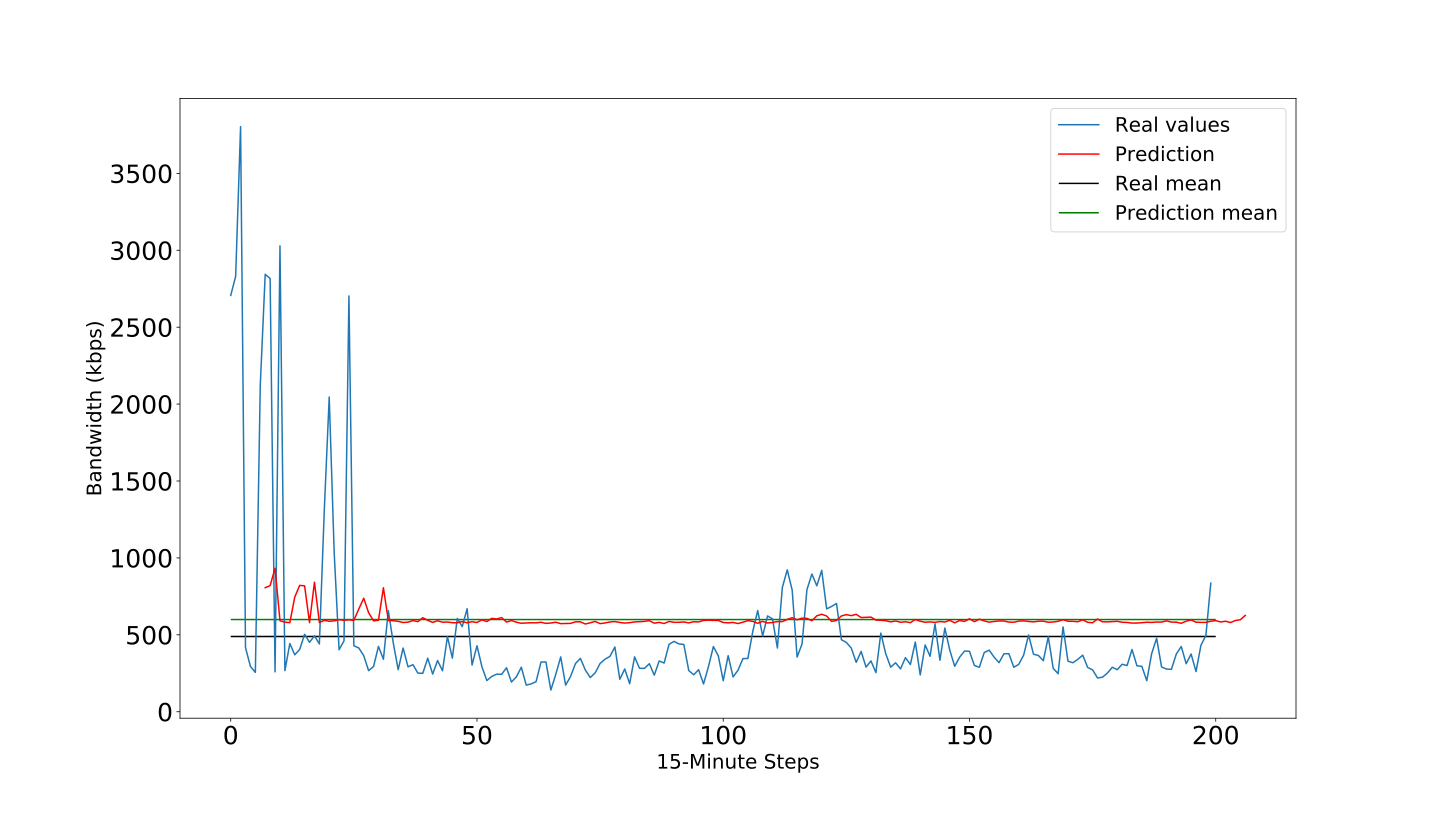
\includegraphics[width=1\linewidth]{Pictures/BigStep/LSTM_Big_Step_81}
		\caption{8 Steps into the future}
		\label{fig:bigStep8}
	\end{subfigure}
	\begin{subfigure}{1\linewidth}
		\centering
		\includegraphics[width=1\linewidth]{Pictures/BigStep/LSTM_Big_Step_161}
		\caption{16 Steps into the future}
		\label{fig:bigStep16}
	\end{subfigure}
	\caption{The prediction of an LSTM predicting 8 and 16 steps into the future.}
	\label{fig:bigStep1}
\end{figure}

\begin{figure}
	\centering
	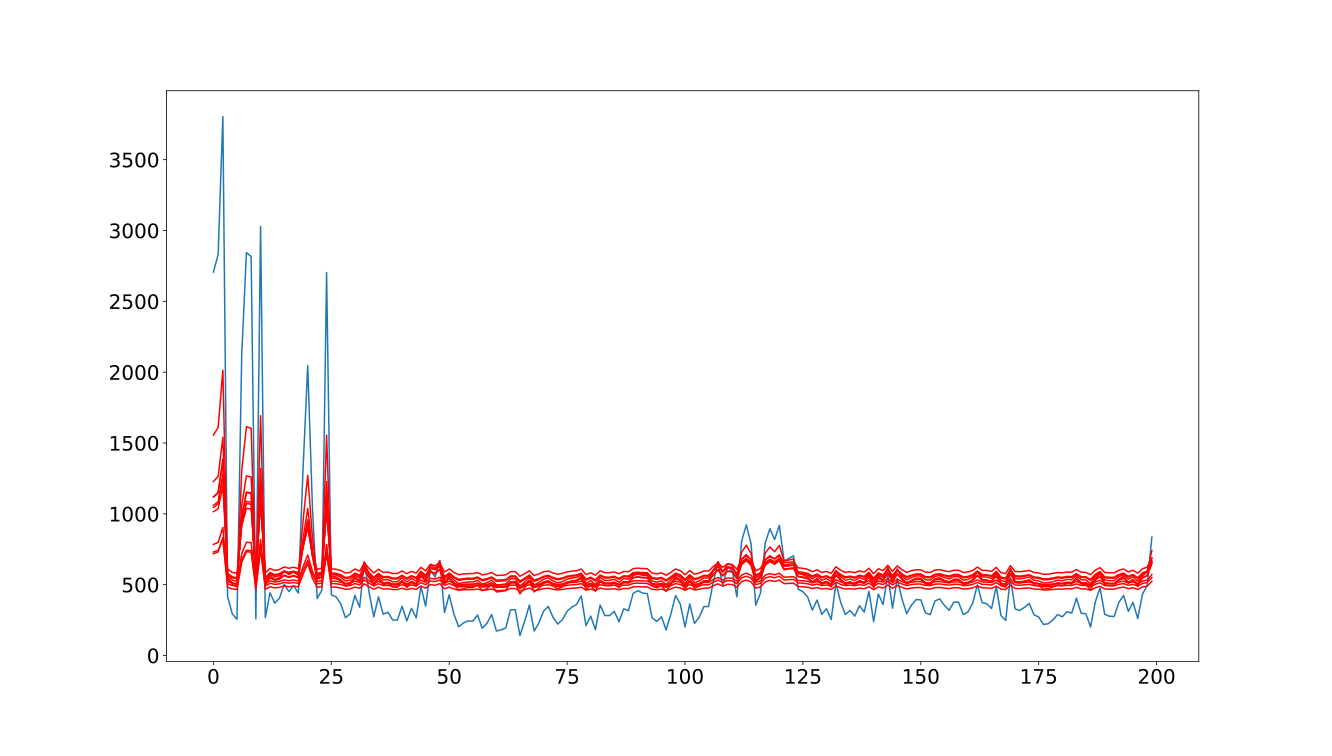
\includegraphics[width=1\linewidth]{Pictures/RangePrediction/LSTM_Range_1}
	\caption{10 values predicted at the same time plotted without shift.}
	\label{fig:lstmrange1}
\end{figure}
